\chapter{DESENVOLVIMENTO}
\label{c.Desenvolvimento}

O desenvolvimento do projeto dividiu-se em quatro fases: a montagem do ambiente de testes de assinaturas construídas a partir de regras do Yara; a obtenção das regras e construção de um índice de agrupamento das mesmas para agilizar a execução das varreduras; obtenção e escolha de amostras de \textit{malware} para testagem; bateria de testes final e análise de resultados. Complementarmente, foi desenvolvida a ideia de uma aplicação \textit{web} para análise de \textit{malware} com base em regras de detecção do Yara.

\section{Obtenção das regras de detecção}
\label{s.obtregras}


\section{Testes iniciais com o ambiente de desenvolvimento}
\label{s.testesiniciais}

\section{Testagem completa e análise de resultados}
\label{s.testefull}

\section{Ideia de uma aplicação web do projeto desenvolvido}
\label{s.prototipo}

\begin{figure}
  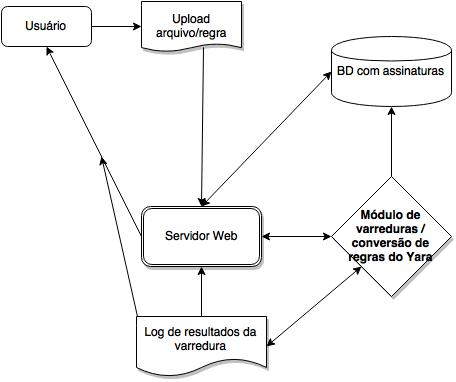
\includegraphics{/figs/flux_prototipo}
  \caption{Fluxograma de funcionamento da aplicação. Fonte: elaborada pelo autor.}
  \label{f.flux_prototipo}
\end{figure}

% - Testes iniciais [ x ]

% - Testagem completa e análise de resultados [ ]

% - Ideia da aplicação web e desenvolvimento parcial do sistema []
